\section{Auswertung}
\label{sec:Auswertung}
\subsection{Verifizieren der Linsengleichung}
Um die Gleichung \ref{eqn:V} und \ref{eqn:D} zu verifizieren sind die dafür Relevanten Messwerte in Tabelle \ref{tab:VdA} aufgetragen. Die Gegenstandsgröße $G$ des Pearl L beträgt $3.0 \cdot 10^{-2}$ m und die Vergrößerungen werden entsprechen $V_1 = \frac{b}{g}$ und $V_2 = \frac{B}{G}$ berechnet.
\begin{table}
  \centering
  \begin{tabular}{c c c c c c}
    \toprule
    $g / 10^{-2}$ m & $b / 10^{-2}$ m & $B / 10^{-3}$ m & $V_1$ & $V_2$ & $\left\lvert \frac{V_1 - V_2}{V_1} \right\rvert / \% $\\
   \midrule
    25	& 15.6	& 2.0 	& 0.62 & 0.66	& 6.6 	\\
    24	& 16.4	& 2.0	& 0.68 & 0.66	& 3.0	\\
    23	& 16.8	& 2.2	& 0.73 & 0.73	& 0.0	\\
    22	& 17.6	& 2.3	& 0.80 & 0.77	& 3.8	\\
    21	& 18.4	& 2.7	& 0.88 & 0.90	& 2.3	\\
    20	& 19.3	& 2.8	& 0.97 & 0.93	& 4.1	\\
    19	& 20.5	& 3.1	& 1.08 & 1.03	& 4.7	\\
    18	& 21.4	& 3.4	& 1.18 & 1.13	& 4.2	\\
    17	& 23.1	& 4.2	& 1.35 & 1.40	& 3.7	\\
    16	& 25.1	& 4.7	& 1.56 & 1.57	& 0.6	\\
    15	& 29.2	& 5.7	& 1.94 & 1.90	& 2.1	\\
    \bottomrule
  \end{tabular}
  \caption{Verifizierung des Abbildungsgesetzes}
  \label{tab:VdA}
\end{table}
\subsection{Bestimmung einer Bekannten sowie Unbekannten Brennweite}
Desweiteren wird zur Ermittlung der Brennweite ein Plot erstellt, wobei die Gegenstandsweiten auf die Y-Achse des Koordinatensystems aufgetragen werden und mit den entsprechenden Bildweiten, welche auf der X-Achse aufgetragen sind, verbunden. Aus dem Schnittpunkt der Graden lässt sich die Brennweite der Linse Ablesen. Aus Abbildung \ref{fig:fibek} wird die Brennweite
\begin{equation}
  f_\text{abgelesen} = (\num{9.8 +- 0.7}) 10^{-2} \, \text{m}
  \label{eqn:fbek}
\end{equation} abgelesen. 
\begin{figure}
  \centering
  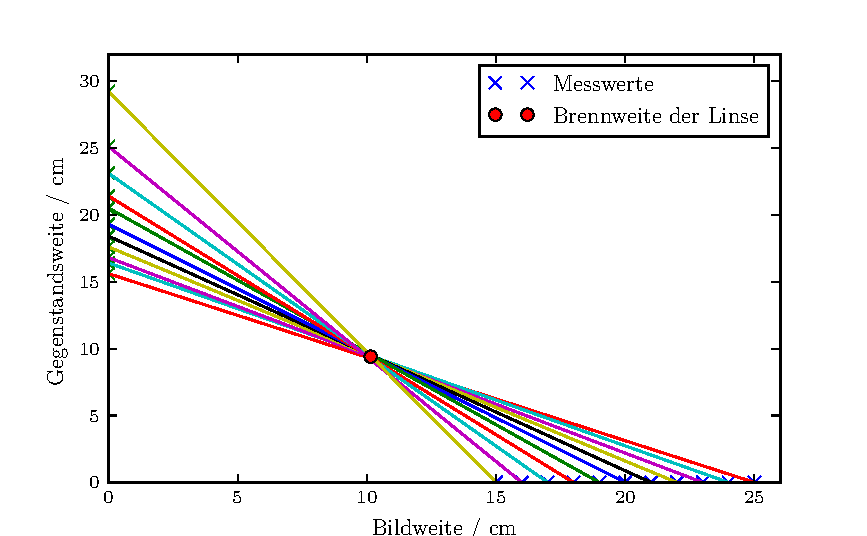
\includegraphics[height=5cm]{bekannt.pdf}
  \caption{Brennweite einer bekannten Linse}
  \label{fig:fibek}
\end{figure}
Die vom Herstelller angegeben Brennweite beträgt 
\begin{equation}
  f_\text{Hersteller} = 10\cdot10^{-2}  \, \text{m} \, .
  \label{eqn:fHer}
\end{equation}
Die Messung wird für eine Linse mit unbekannter Brechkraft wiederhholt und aus dem Diagramm \ref{fig:fiunb} lässt sich eine Brennweite von 
\begin{equation}
  f_\text{unbekannt} = (\num{11.9 +- 4.6}) \, \text{m}
  \label{eqn:unb}
\end{equation}
ablesen.
\begin{figure}
  \centering
  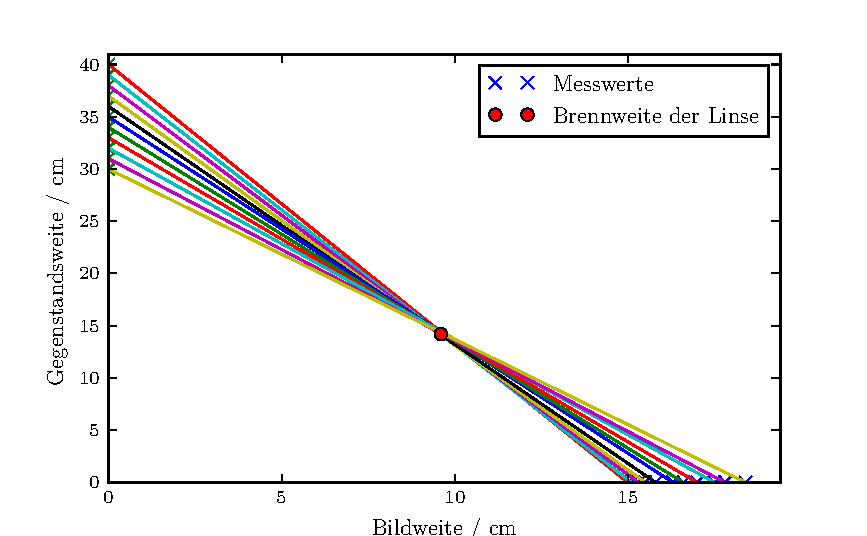
\includegraphics[height=5cm]{unbekannt.pdf}
  \caption{Brennweite einer unbekannten Linse}
  \label{fig:fiunb}
\end{figure}

\subsection{Besselmethode}
Die entsprechenden Messdaten zu dem Versuch sind in Tabelle \ref{tab:ffw} zu finden.  Dabei wirde die Brennweite nach Formel \ref{eqn:tbes} berechnet, wobei der Abstand $d = g - b$ und die Gegenstandsweite als $g = e - b$ dem enstsprechend definiert ist.
\begin{table}
  \centering
  \begin{tabular}{c c c | c c}
    \toprule
    $e$ / $10^{-2}$ m & $g_1$ / m & $g_2$ / m & $f$ / $10^{-2}$ m & $f$ / $10^{-2}$ m\\
    \midrule
	100.0	& 11.5	& 89.3	& 10.18	& 9.48	\\
	97.5	& 11.5	& 86.9	& 10.14	& 9.41	\\
	95.0	& 11.6	& 84.4	& 10.18	& 9.61	\\
	92.5	& 11.6	& 81.6	& 10.15	& 9.58	\\
	90.0	& 11.7	& 79.1	& 10.18	& 9.61	\\
	87.5	& 11.7	& 76.5	& 10.14	& 8.74	\\	
	85.0	& 11.8	& 75.1	& 10.16	& 7.94	\\	
	82.5	& 11.9	& 73.6	& 10.18	& 9.56	\\
	80.0	& 11.9	& 68.9	& 10.13	& 9.51	\\
	77.5	& 12.1	& 66.4	& 10.21	& 9.37	\\
   \midrule
		&	&	& \num{10.16 +- 0.01} & \num{9.3 +- 0.1} \\
   \bottomrule
  \end{tabular}
  	\caption{Brennweite von weißem Licht}
  \label{tab:ffw}
\end{table}
Aus Mittlung der Einzelmesswerte erhält man durch die Besselmethode eine experimentell bestimmte Brennweite von 
\begin{equation}
  f_\text{exp} = (\num{9.7 +- 0.1}) 10^{-2} \, \text{m} \ .
  \label{eqn:fexp}
\end{equation}
Für den Versuch wurde eine Brennweite von 
\begin{equation}
  f_\text{Hersteller} = 10 \cdot 10^{-2} \, \text{m}
  \label{eqn:fHer}
\end{equation}
verwendet.
Anschließend wird die Brechkraft von farbigen Licht bestimmt. Dazu wird zunächst ein roter und anschließend ein blauer Farbfilter vor die Lampe gespannt.
\begin{table}
  \centering
  \begin{tabular}{c | c c c || c c c}
    \toprule
    $e$ / m & $g_\text{rot} / 10^{-2}$ m & $b_\text{rot} / 10^{-2}$ m & $f_\text{rot} / 10^{-2}$ m & $g_\text{blau} / 10^{-2}$ m & $b_\text{blau} / 10^{-2}$ m & $f_\text{blau} / 10^{-2}$ m \\
    \midrule
    100	& 89.3	& 10.7	& 9.6 &	89.3 & 10.7 & 9.6	\\
    90	& 79.1	& 10.9	& 9.6 & 79.3 & 10.7 & 9.4	\\
    80	& 68.8	& 11.2	& 9.6 & 69.0 & 11.0 & 9.5	\\
    70	& 58.5	& 11.5	& 9.6 & 58.6 & 11.4 & 9.4	\\
    60	& 48.0	& 12.0	& 9.6 & 48.4 & 11.6 & 9.4	\\
    \bottomrule
  \end{tabular}
  \caption{Brennweite von rotem und blauem Licht}
  \label{tab:fbesslf}
\end{table}
Aus der Tabelle \ref{tab:fbesslf} ergibt sich für rotes Licht eine Brennweite von
\begin{equation}
  f_\text{rot} = (\num{9.60 +- 0.01}) \, 10^{-2} \, \text{m}
  \label{eqn:frot}
\end{equation} 
und für blaues Licht eine Brennweite von 
\begin{equation}
  f_\text{blau} = (\num{9.49 +- 0.02}) \, 10^{-2} \, \text{m} \ .
  \label{fblau}
\end{equation}

\subsection{Methode nach Abbe}
Es sollen die Hauptebene und die Brennweite mit hilfe der Formeln \ref{eqn:g'} und \ref{eqn:b'} bestimmt werden. Dafür wird zunächst eine lineare Regression durchgeführt und die Fitparameter sich ausgegeben gelassen. 
\begin{figure}
  \centering
    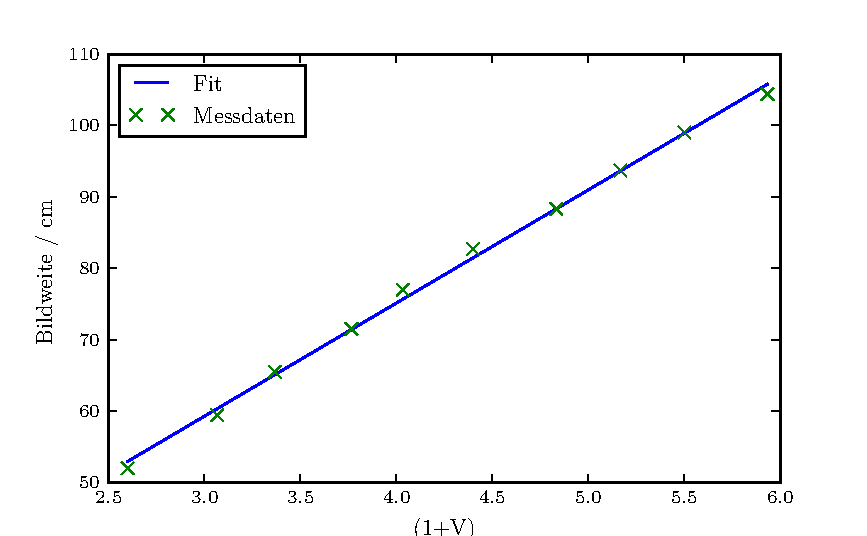
\includegraphics[height=5cm]{Abbe1.pdf}
  \caption{Gegenstandsweiten Fit}
  \label{fig:<+label+>}
\end{figure}
\begin{figure}
  \centering
  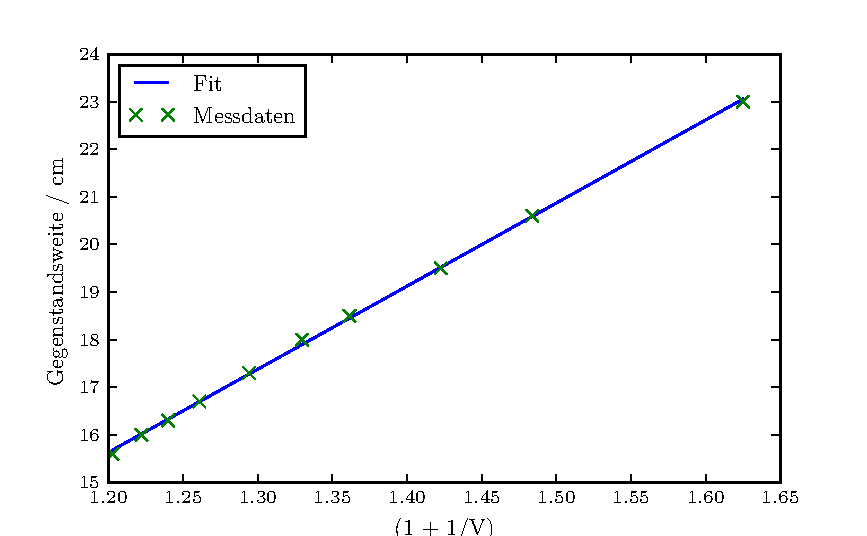
\includegraphics[height=5cm]{Abbe2.pdf}
  \caption{Bildweiten Fit}
  \label{fig:<+label+>}
\end{figure}
Der Fit ergibt die Brennweiten und die Laage der Hauptebenen
\begin{eqnarray}
  f_\text{g} &= (\num{ 15.9 +- 0.3}) \cdot 10^{-2} \, \text{m} \\ 
  f_\text{b} &= (\num{ 17.5 +- 0.1 }) \cdot 10^{-2} \, \text{m} \\
  h &= (\num{ 11 +- 1}) \cdot 10^{-2} \, \text{m} \\
  h' &= (\num{ -5.3 +- 0.18}) \cdot 10^{-2} \,\text{m} 
  \label{eqn:abbedf}
\end{eqnarray}
